\section{Physics Case Study}\hfill

To demonstrate that the model is able to provide useful insight into a practical physics analysis, we attempt to reconstruct the Higgs boson mass from the simulated di-Higgs dataset along with a non-resonant multijet background sample (denoted 4b). 

\begin{figure}[ht]
\centering
\begin{subfigure}{.32\textwidth}
  \centering
  \textbf{\tiny{Raw Mass $\left \langle \mu \right \rangle=200$}}
  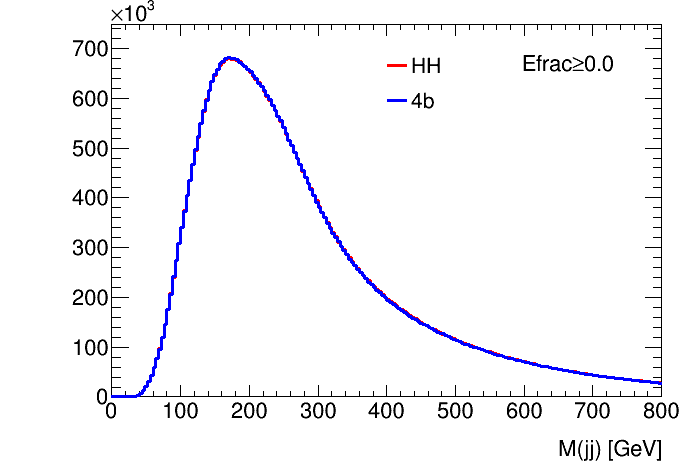
\includegraphics[width=1\linewidth]{mass_peak_nocut.png}
  \caption{}
  \label{fig:Raw}
\end{subfigure}
\begin{subfigure}{.32\textwidth}
  \centering
  \textbf{\tiny{Uncorrected Mass $\left \langle \mu \right \rangle=200$}}
  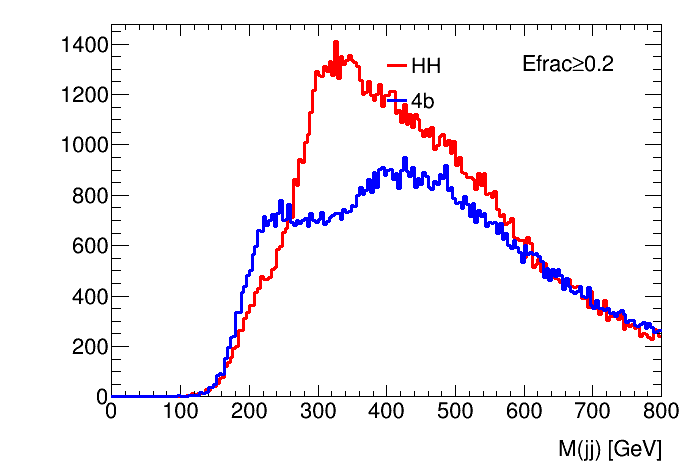
\includegraphics[width=1\linewidth]{mass_peak_uncorrected.png}
  \caption{}
  \label{fig:Uncorrected}
\end{subfigure}
\begin{subfigure}{.32\textwidth}
  \centering
  \textbf{\tiny{Corrected Mass $\left \langle \mu \right \rangle=200$}}
  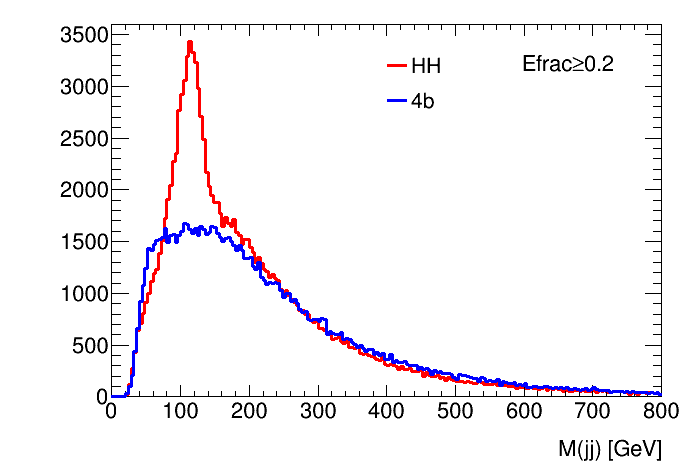
\includegraphics[width=1\linewidth]{mass_peak_corrected.png}
  \caption{}
  \label{fig:Corrected}
\end{subfigure}
\caption{The reconstructed Higgs boson mass when looking at (a) all jets with no cuts on $E_{frac}$ and no corrections, (b) uncorrected jets with cut at true $E_{frac}>0.2$, and (c) corrected jets (according to model predictions) with cut at predicted $E_{frac}>0.2$. (a) Shows no signs of mass peak due to pileup contamination. (b) Shows a mass peak that is heavily smeared due to pileup. (c) Shows the expected narrow narrow peak near $m_{\rm H}\approx 125$~GeV with corrections applied.}
\label{fig:MassPeak}
\end{figure}

The background sample was generated as the MadGraph process\newline\texttt{p p > b b\~{} b b\~{}} with the minimum $p_{\rm T}$ of the $b$-quarks set to 60~GeV to ensure the same kinematics of both samples, so that the only visible difference between the samples is the resonant mass peak that appears in the di-Higgs sample. Figure \ref{fig:MassPeak} shows the reconstructed mass of all possible pairs of jets in each event, and we expect to find a resonance mass peak near $m_{\rm H}\approx 125$~GeV with a narrow width. Figure \ref{fig:Raw} shows the uncorrected jets with no cut applied to $E_{frac}$ and the background and signal are indistinguishable. Figure \ref{fig:Uncorrected} shows that a cut at truth level $E_{frac}>0.2$ shows a resonant mass peak with uncorrected jets, however, the mean and the width of the mass peak has been significantly inflated due to the effects of pileup. Figure \ref{fig:Corrected} shows that a cut a prediction level $E_{frac}>0.2$ on corrected jets shows a mass peak near the expected value of 125~GeV with a narrow width which shows that the use of $E_{frac}$ and $M_{frac}$ to correct jets successfully mitigates the effects of pileup and restores physical quantities to their expected values.

Lastly, we would like to show that one can slightly modify the learning objective of the model to directly classify an event as signal or background through a binary classification task, which circumvents the need for computationally costly combinatorics. To demonstrate this effect, a self-encoder module between jets is trained on a binary classification task, di-Higgs vs 4b, for three different cases where jets are represented by the following features: (1) $[p_{\rm T},\eta,\phi,m]$, (2) $[p_{\rm T},\eta,\phi,m,E_{frac}^{pred}, M_{frac}^{pred}]$, and (3) $[p_{\rm T},\eta,\phi,m,E_{frac}^{true}, M_{frac}^{true}]$. Through learning the proper attention weights between jets, the model is able to perceive the mass peak and directly classify the event as di-Higgs signal or 4b background. Figure \ref{fig:ROC} shows the background rejection, the reciprocal of false positive rate, vs the signal efficiency, the true positive rate. 

\begin{figure}[h]
\centering
\begin{subfigure}{.55\textwidth}
  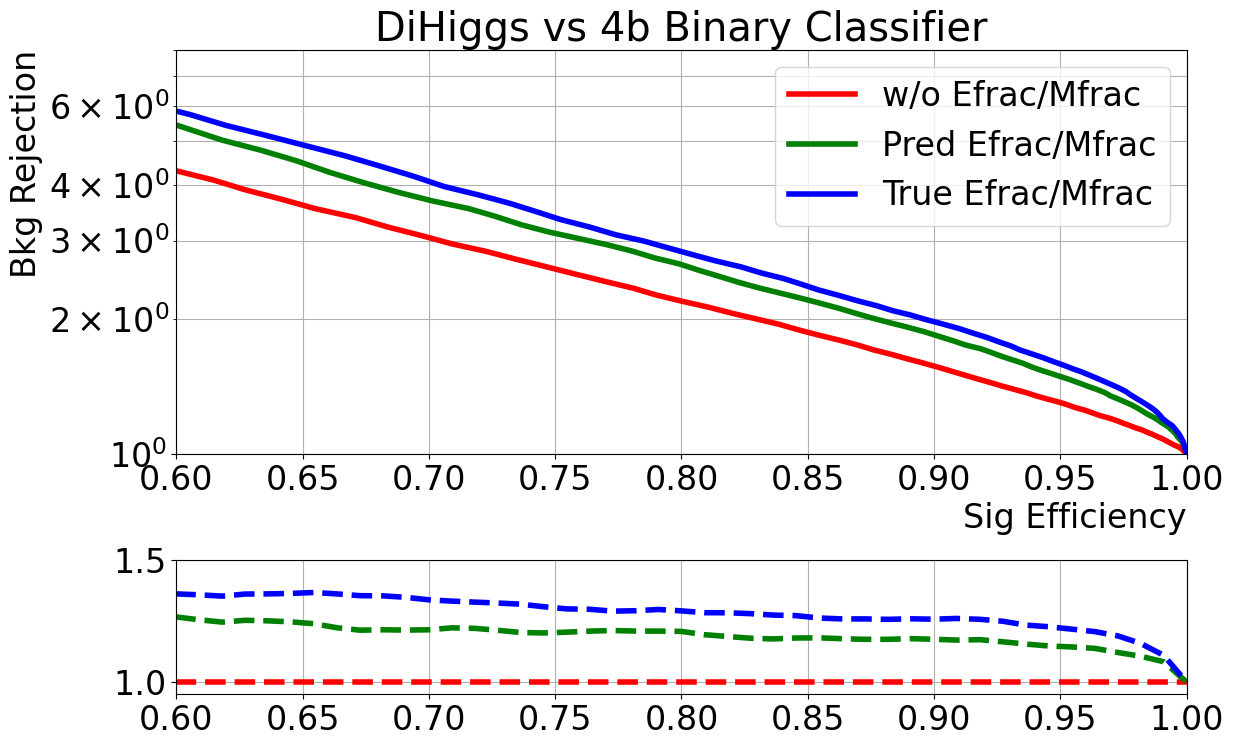
\includegraphics[width=1\linewidth]{Analysis_ROC.png}
  \caption{}
  \label{fig:ROC}
\end{subfigure}%
\begin{subfigure}{.43\textwidth}
  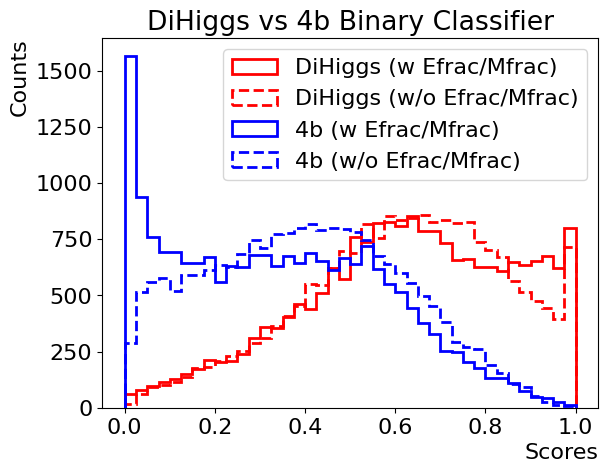
\includegraphics[width=1\linewidth]{Analysis_Scores.png}
  \caption{}
  \label{fig:Scores}
\end{subfigure}
\caption{For the purposes of physics analysis, the learning objective is modified to perform direct binary classification of di-Higgs vs 4b. $E_{frac}$ and $M_{frac}$ improve performance of the classifier.}
\label{fig:Analysis}
\end{figure}

For the case (1) \myname{} is able to successfully distinguish between di-Higgs and 4b physics processes despite having quite similar kinematic features. When predicted and truth $E_{frac}$ and $M_{frac}$ are provided in case (2) and (3), respectively, \myname{} has a noticeable increase in background rejection. This improvement is elucidated in Figure \ref{fig:Scores} where the dashed line represents case (1) and the solid lines represent case (2). Here one can see a dramatic improvement in the lowest bin, background-like, and highest bin, signal-like which proves the the predicted $E_{frac}$ and $M_{frac}$ of the model can be used directly to perform event level classification.

